% Cohen-Lenstra probabilities p=3 vs cokernels of 20000 random 12x12 matrices over Z/81 (generated by a script).
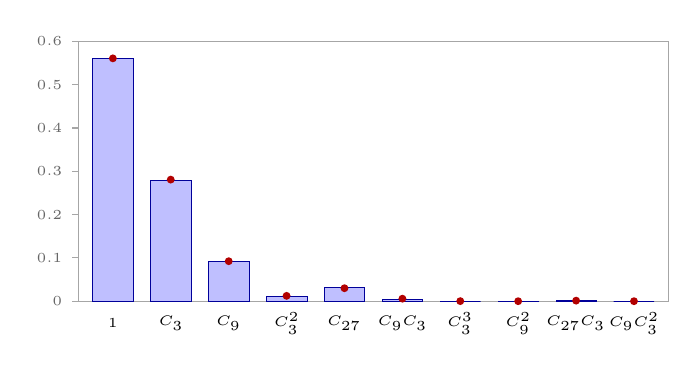
\begin{tikzpicture}[x=1cm,y=1cm]
\draw[black!35] (0,0) rectangle (7.50,3.30);
\draw[black!35] (0,0.00)--(-0.08,0.00) node[left,font=\tiny,black!60]{$0$};
\draw[black!35] (0,0.55)--(-0.08,0.55) node[left,font=\tiny,black!60]{$0.1$};
\draw[black!35] (0,1.10)--(-0.08,1.10) node[left,font=\tiny,black!60]{$0.2$};
\draw[black!35] (0,1.65)--(-0.08,1.65) node[left,font=\tiny,black!60]{$0.3$};
\draw[black!35] (0,2.20)--(-0.08,2.20) node[left,font=\tiny,black!60]{$0.4$};
\draw[black!35] (0,2.75)--(-0.08,2.75) node[left,font=\tiny,black!60]{$0.5$};
\draw[black!35] (0,3.30)--(-0.08,3.30) node[left,font=\tiny,black!60]{$0.6$};
\node[font=\tiny] at (0.44,-0.28) {$1$};
\node[font=\tiny] at (1.18,-0.28) {$C_3$};
\node[font=\tiny] at (1.91,-0.28) {$C_9$};
\node[font=\tiny] at (2.65,-0.28) {$C_3^2$};
\node[font=\tiny] at (3.38,-0.28) {$C_{27}$};
\node[font=\tiny] at (4.12,-0.28) {$C_9C_3$};
\node[font=\tiny] at (4.85,-0.28) {$C_3^3$};
\node[font=\tiny] at (5.59,-0.28) {$C_9^2$};
\node[font=\tiny] at (6.32,-0.28) {$C_{27}C_3$};
\node[font=\tiny] at (7.06,-0.28) {$C_9C_3^2$};
\filldraw[blue!25,draw=blue!60!black,line width=0.2pt] (0.184,0) rectangle (0.699,3.081);
\filldraw[blue!25,draw=blue!60!black,line width=0.2pt] (0.919,0) rectangle (1.434,1.540);
\filldraw[blue!25,draw=blue!60!black,line width=0.2pt] (1.654,0) rectangle (2.169,0.513);
\filldraw[blue!25,draw=blue!60!black,line width=0.2pt] (2.390,0) rectangle (2.904,0.064);
\filldraw[blue!25,draw=blue!60!black,line width=0.2pt] (3.125,0) rectangle (3.640,0.171);
\filldraw[blue!25,draw=blue!60!black,line width=0.2pt] (3.860,0) rectangle (4.375,0.029);
\filldraw[blue!25,draw=blue!60!black,line width=0.2pt] (4.596,0) rectangle (5.110,0.000);
\filldraw[blue!25,draw=blue!60!black,line width=0.2pt] (5.331,0) rectangle (5.846,0.001);
\filldraw[blue!25,draw=blue!60!black,line width=0.2pt] (6.066,0) rectangle (6.581,0.010);
\filldraw[blue!25,draw=blue!60!black,line width=0.2pt] (6.801,0) rectangle (7.316,0.000);
\fill[red!70!black] (0.441,3.084) circle (0.05cm);
\fill[red!70!black] (1.176,1.544) circle (0.05cm);
\fill[red!70!black] (1.912,0.508) circle (0.05cm);
\fill[red!70!black] (2.647,0.068) circle (0.05cm);
\fill[red!70!black] (3.382,0.165) circle (0.05cm);
\fill[red!70!black] (4.118,0.032) circle (0.05cm);
\fill[red!70!black] (4.853,0.001) circle (0.05cm);
\fill[red!70!black] (5.588,0.000) circle (0.05cm);
\fill[red!70!black] (6.324,0.007) circle (0.05cm);
\fill[red!70!black] (7.059,0.000) circle (0.05cm);
\end{tikzpicture}
